%
%
%

\begin{frame}[t, allowframebreaks]{Precursors of Artifial Intelligence -}

    \vspace{-0.1cm}
    We have always dreamt of building machines with human-like intelligence!\\
    \begin{itemize}
        \small
        \item
        We have myths and stories of master craftsmen and intelligent machines.\\
    \end{itemize}
    \vspace{-0.4cm}

    \begin{columns}[t]
        \begin{column}{0.46\textwidth}
         \begin{center}
          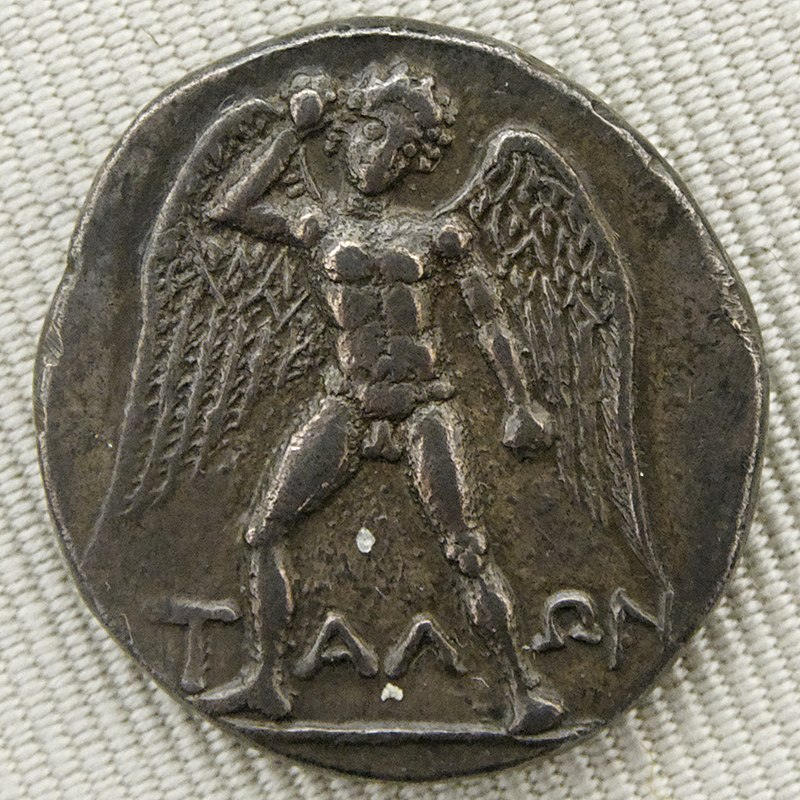
\includegraphics[width=0.99\textwidth]{./images/precursors/talos.jpg}\\
          {\scriptsize 
          \vspace{0.1cm}
          Talos on a Greek coin from 300 BCE.\\
          \color{col:attribution} 
          (Cabinet des Médailles, Paris.)
          \href{https://en.wikipedia.org/wiki/Talos\#/media/File:Didrachm_Phaistos_obverse_CdM.jpg}{\tiny [link]}
          \\}
         \end{center}
        \end{column}
        \begin{column}{0.54\textwidth}
            \begin{itemize}
                \small
                \item 
                {\bf Talos}, the bronze giant built by the god
                Hephaestus to protect Crete from invaders.
                \href{https://en.wikipedia.org/wiki/Talos}{\tiny [Wikipedia]}
                \item 
                {\bf Galatea}, the female ivory statue animated 
                by the goddess Aphrodite when its sculptor, Pygmalion, 
                fell in love with it.
                \href{https://en.wikipedia.org/wiki/Pygmalion_(mythology)}{\tiny [Wikipedia]}
                \item
                {\bf Golems} in Jewish folklore, made from clay 
                and animated by words written on their foreheads, 
                or on pieces of paper placed in their mouth.
                \href{https://en.wikipedia.org/wiki/Golem}{\tiny [Wikipedia]}
                \item
                {\bf Homunculi} (sing.: Homunculus), 
                the little anthropomorphic creatures found in alchemical traditions.
                \href{https://en.wikipedia.org/wiki/Homunculus}{\tiny [Wikipedia]}
            \end{itemize}        
        \end{column}
    \end{columns}

    \framebreak

    \begin{itemize}
        \small
        \item
        {\bf Brazen heads}, the future-telling automata of 
        Gerbert of Aurillac, Saint Albertus, Robert Grosseteste, 
        and Roger Bacon.
        \href{https://en.wikipedia.org/wiki/Brazen_head}{\tiny [Wikipedia]}\\
        \item
        {\bf Frankenstein!} by Marry Shelley (1818).
        
\includegraphics[width=0.04\textwidth]{./images/precursors/stein.jpg}
        \href{https://en.wikipedia.org/wiki/Frankenstein}{\tiny [Wikipedia]}\\
        \item
        {\bf Hadaly}, the female android in the science fiction novel `The Future Eve' (1886)
        by Auguste Villiers de I'Isle-Adam.
        \href{https://en.wikipedia.org/wiki/The_Future_Eve}{\tiny [Wikipedia]}\\
        \item
        {\bf Maria} in the science fiction movie `Metropolis' (1927)
        \href{https://en.wikipedia.org/wiki/Metropolis_(1927_film)}{\tiny [Wikipedia]}\\
    \end{itemize}        

    \vspace{-0.3cm}

    \begin{columns}[t]
        \begin{column}{0.32\textwidth}
            \begin{center}
                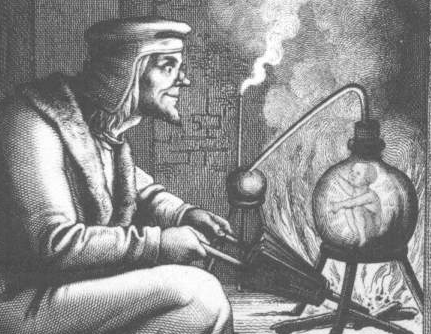
\includegraphics[width=0.99\textwidth]
                {./images/precursors/homunculus_cropped.png}\\
                {\scriptsize 
                \vspace{0.1cm}
                19$^{th}$ century engraving of Wagner and Homunculus 
                from Goethe's Faust II.
                \href{https://en.wikipedia.org/wiki/Homunculus\#/media/File:Faust_image_19thcentury.jpg}{\tiny [link]}\\
                }
            \end{center}
        \end{column}
        \begin{column}{0.37\textwidth}
            \begin{center}
                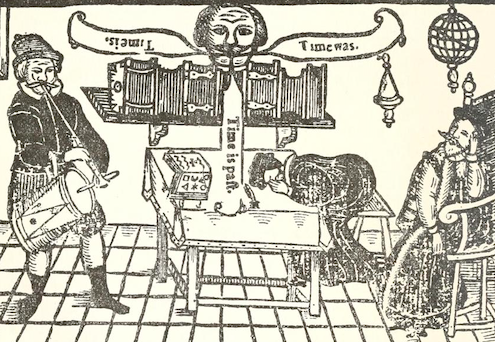
\includegraphics[width=0.99\textwidth]
                {./images/precursors/brazen_head_cropped.png}\\
                {\scriptsize 
                \vspace{0.1cm}
                Reprint of 1630 edition of 
                Robert Greene's Friar Bacon and Friar Bungay.
                \href{https://en.wikipedia.org/wiki/Friar_Bacon_and_Friar_Bungay\#/media/File:Greene_Bacon_and_Bungay_1630.jpg}{\tiny [link]}\\
                }
            \end{center}
        \end{column}
        \begin{column}{0.30\textwidth}
            \begin{center}
                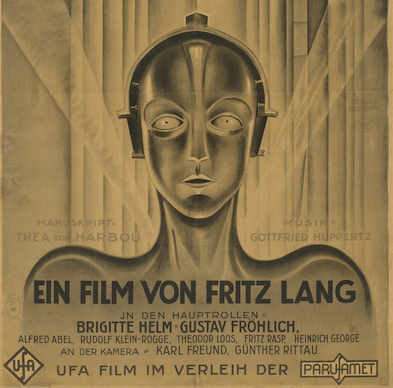
\includegraphics[width=0.80\textwidth]
                {./images/precursors/metropolis_cropped.png}\\
                {\scriptsize 
                \vspace{0.1cm}
                Part of the theatrical release poster for Metropolis,
                by Heinz Schulz-Neudamn.
                \href{https://en.wikipedia.org/wiki/Metropolis_(1927_film)\#/media/File:Metropolis_(German_three-sheet_poster).jpg}{\tiny [link]}\\
                }      
            \end{center}
        \end{column}
    \end{columns}

\end{frame}